\section{The Direct and Indirect Effects of Health Insurance}
\label{sec:healthinsurance}


\begin{figure}[h!]
    \caption{Effects of Health Insurance in the Oregon Health Insurance Experiment.}
    \centering
    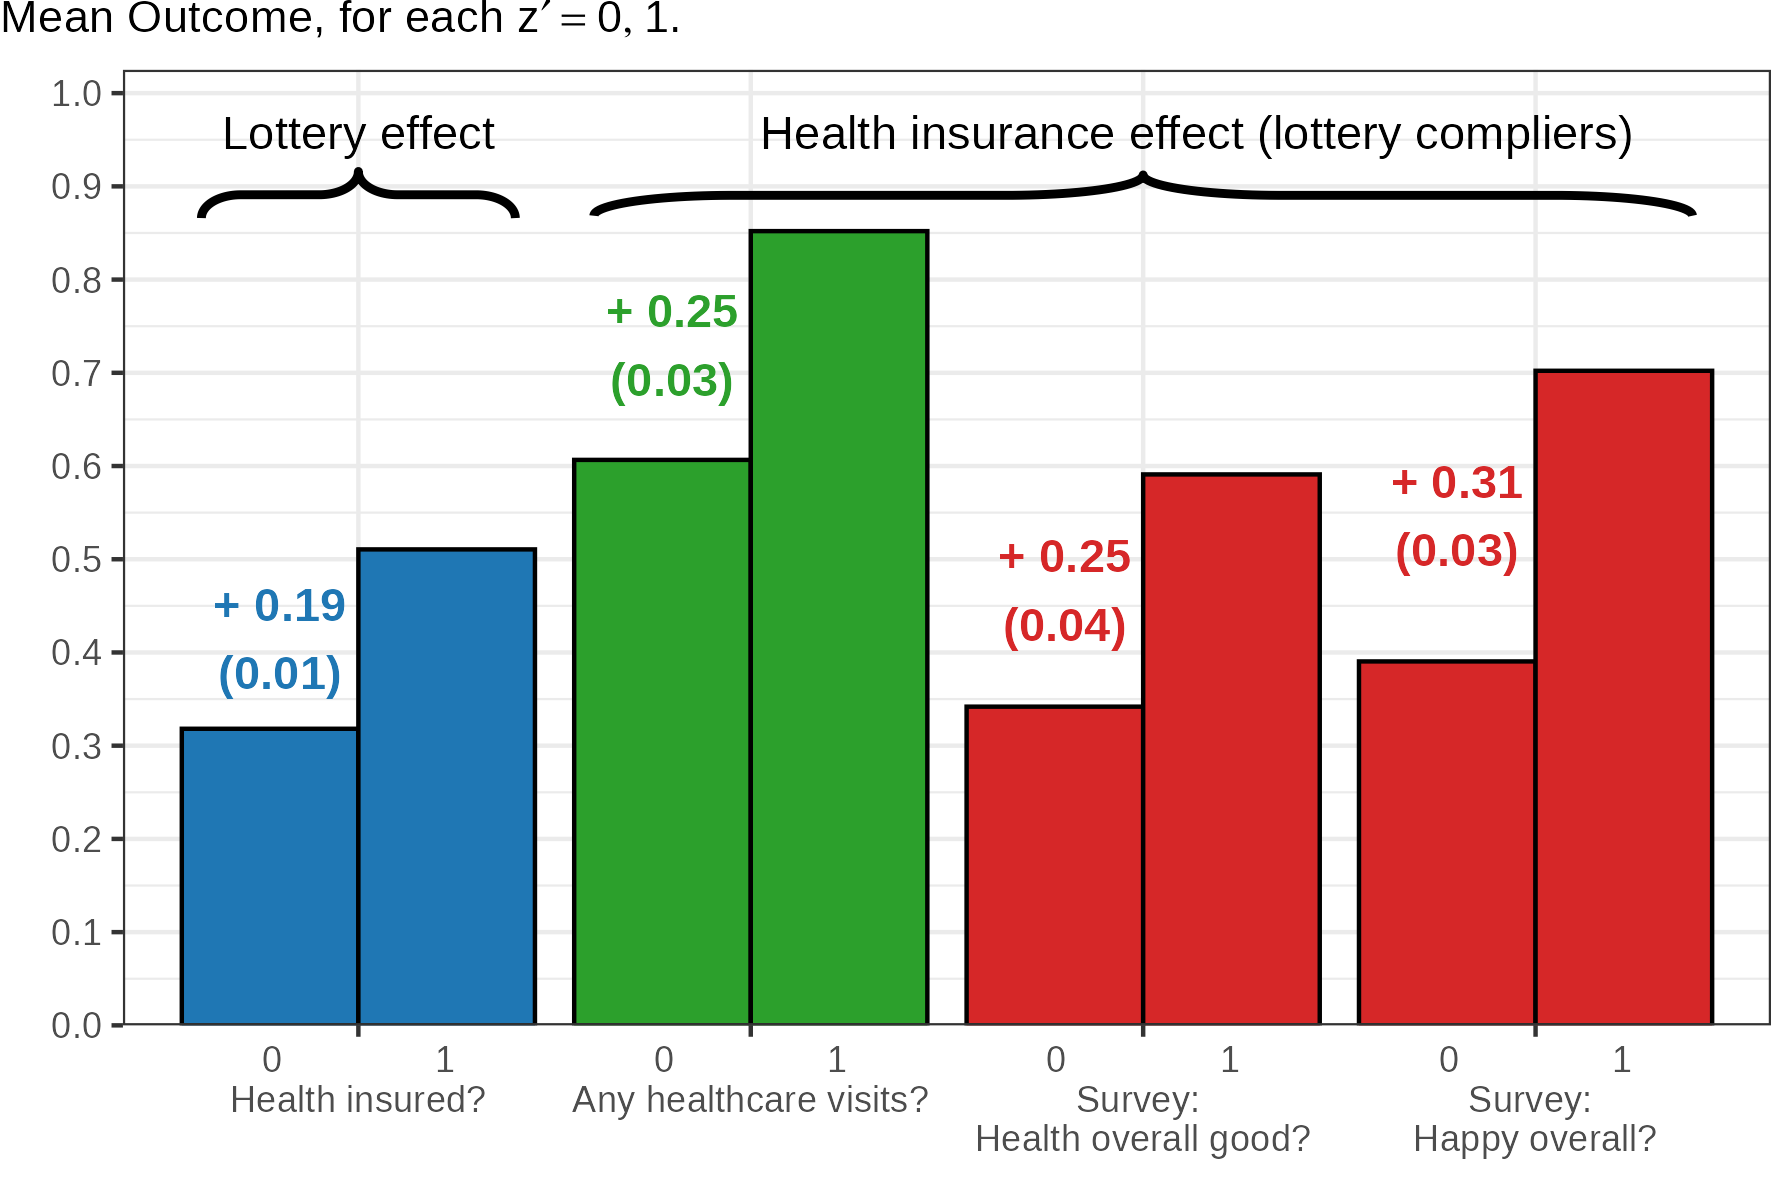
\includegraphics[width=0.85\textwidth]{sections/figures/insurance-effects.png}
    \label{fig:healthinsurance-effects}
    \justify
    \footnotesize    
    \textbf{Note:}
    This figure summarises the relevant results of the Oregon Health Insurance Experiment \citep{finkelstein2008oregon}.
    The lottery results show that being randomly selected off the Medicaid wait-list increased health insurance rate by 19\%.
    The effect of health insurance shows estimates of the avaerage complier effect of having health insurance on surveyed outcomes.
    It uses the wait-list lottery as an instrument for having health insurance, and the \cite{abadie2003semiparametric} weighting scheme to estimate the average complier levels, $\Egiven{Y_i(z',.)}{\text{lottery complier}}$ for each $z'=0,1$.
\end{figure}


\subsection{Accepted Practice in Applied Economics}

Mention the Blackwell paper.
\autoref{appendix:mediation-review} surveys the applied economics literature.
